\documentclass[tikz]{standalone}
% \usepackage{tikz} % already loaded by the documentclass


\begin{document}
%%| caption: A graph of five nodes

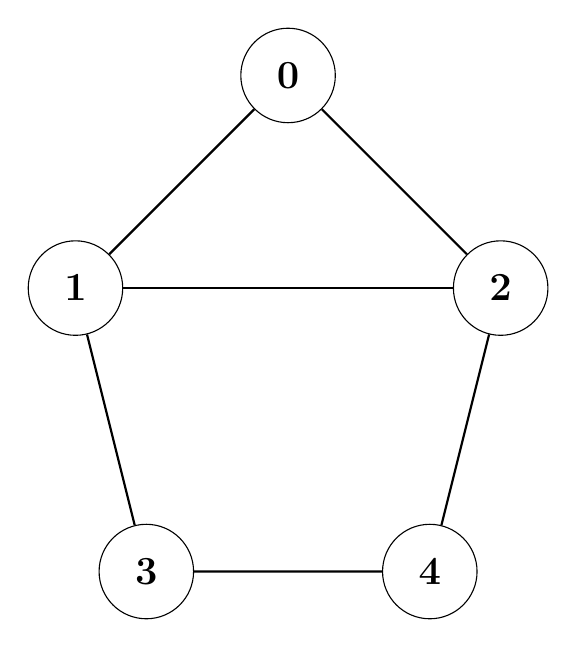
\begin{tikzpicture}[scale=1.8, font=\Large]
  % Define vertices
  \node[circle, draw, fill=white, minimum size=1.2cm] (0) at (0,2) {\textbf{0}};
  \node[circle, draw, fill=white, minimum size=1.2cm] (1) at (-1.5,0.5) {\textbf{1}};
  \node[circle, draw, fill=white, minimum size=1.2cm] (2) at (1.5,0.5) {\textbf{2}};
  \node[circle, draw, fill=white, minimum size=1.2cm] (3) at (-1,-1.5) {\textbf{3}};
  \node[circle, draw, fill=white, minimum size=1.2cm] (4) at (1,-1.5) {\textbf{4}};

  % Draw edges
  \draw[thick, black] (0) -- (1);
  \draw[thick, black] (0) -- (2);
  \draw[thick, black] (1) -- (2);
  \draw[thick, black] (1) -- (3);
  \draw[thick, black] (2) -- (4);
  \draw[thick, black] (3) -- (4);

\end{tikzpicture}
\end{document}
      